For a complete description of the Earth's interior we need to know
it's chemical composition, temperature and pressure.
In section \ref{section_Density-gravity-pressure} 
the pressure is expressed in the density distribution 
and the related internal gravity field.
Once the internal pressure distribution is known,
sharp transitions or discontinuities in the material properties,
like the seismic velocities $v_p, v_s$ and the density 
in the PREM model,
can be identified with mineral phase transitions and as such they can
be related to the mineral $(P,T)$ phase diagram
of candidate mantle silicate materials in order to estimate the temperature 
in the Earth's interior.
Such phase diagrams are determined from
experimental (HPT) and theoretical work in mineral physics.

What do we know about Earth's bulk chemical composition?
Candidate mantle materials have been defined based on
cosmochemical and petrological considerations.
Models of the chemical composition of the Earth are commonly based on
the hypothesis that the planet was formed in a multi-stage accretion proces
from material that condensated from the original solar nebula
approximately 4.6 billion years ago at the time of formation of the
solar system.
The chemical composition of chondritic meteorites, in particular
the carbonaceous chondrites (CI type)
(McBride and Gilmour (2003) \cite{mcgi03})
show a strong correlation with the composition of the outer layer of
the sun (photosphere), determined from spectral analysis of the 
solar light, as illustrated in the following figure:

\begin{center}
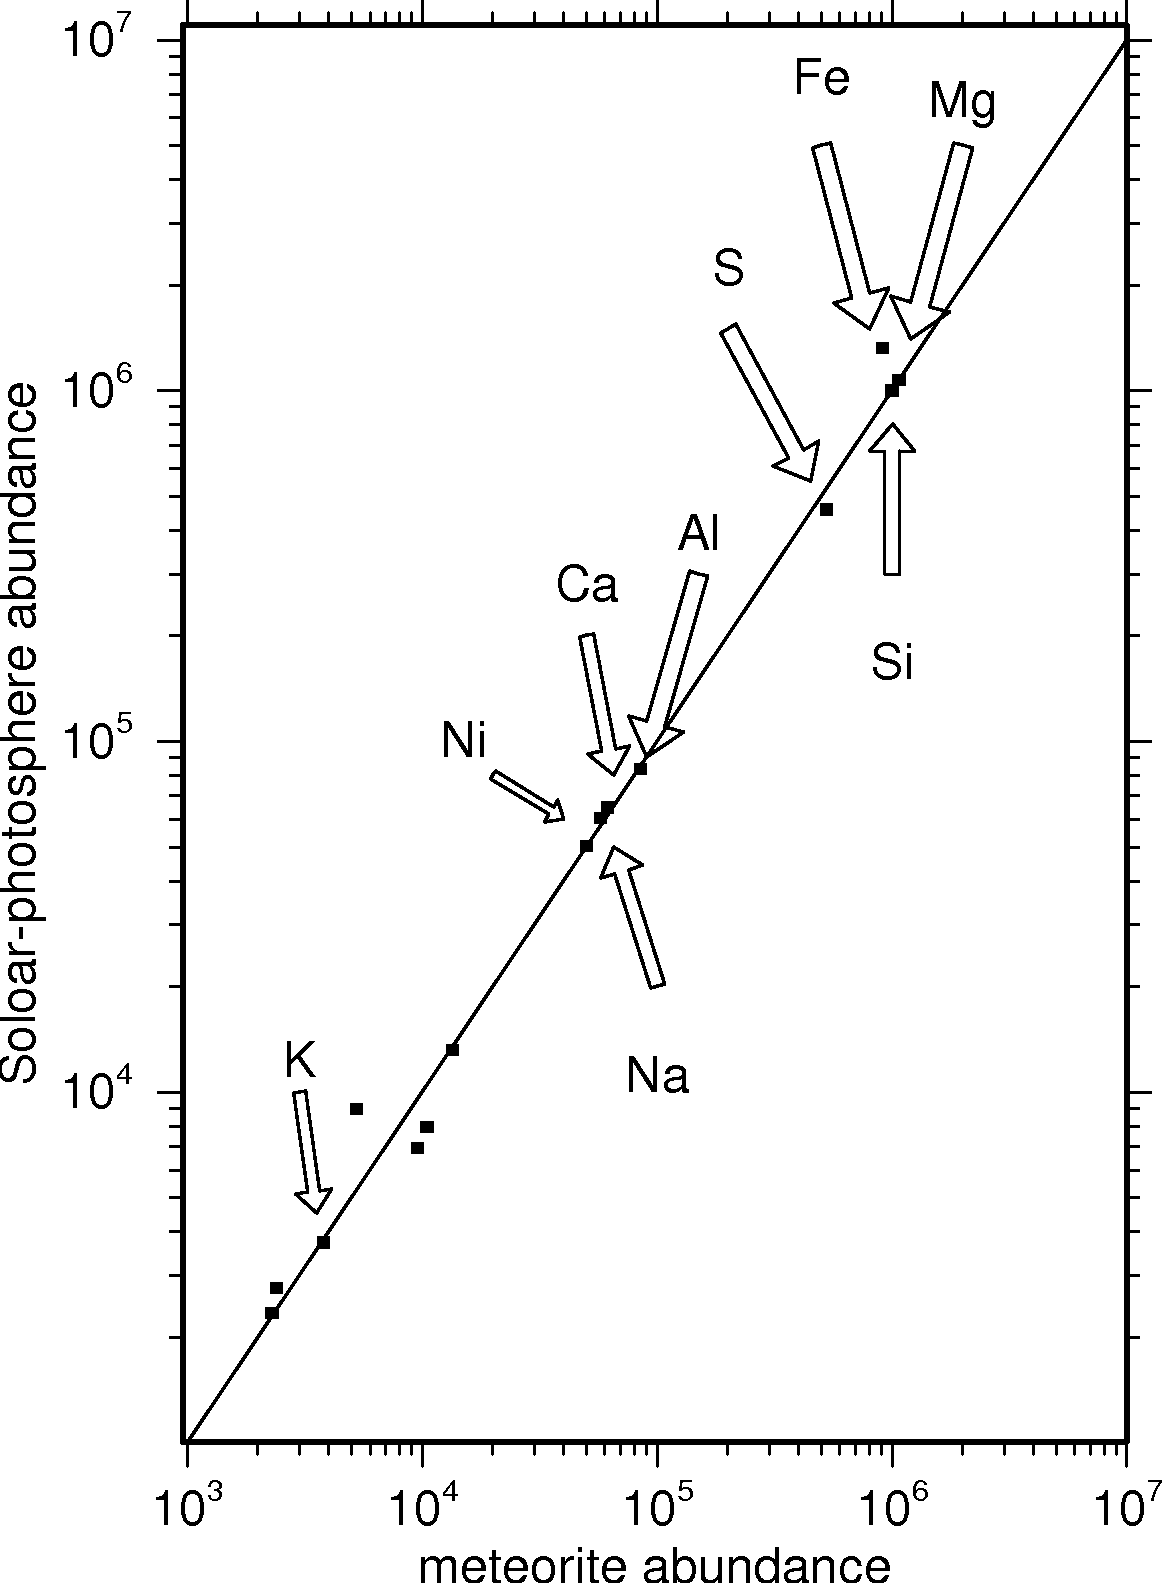
\includegraphics[height=7cm]{images/gravity/photosphere-meteoritic-restricted}
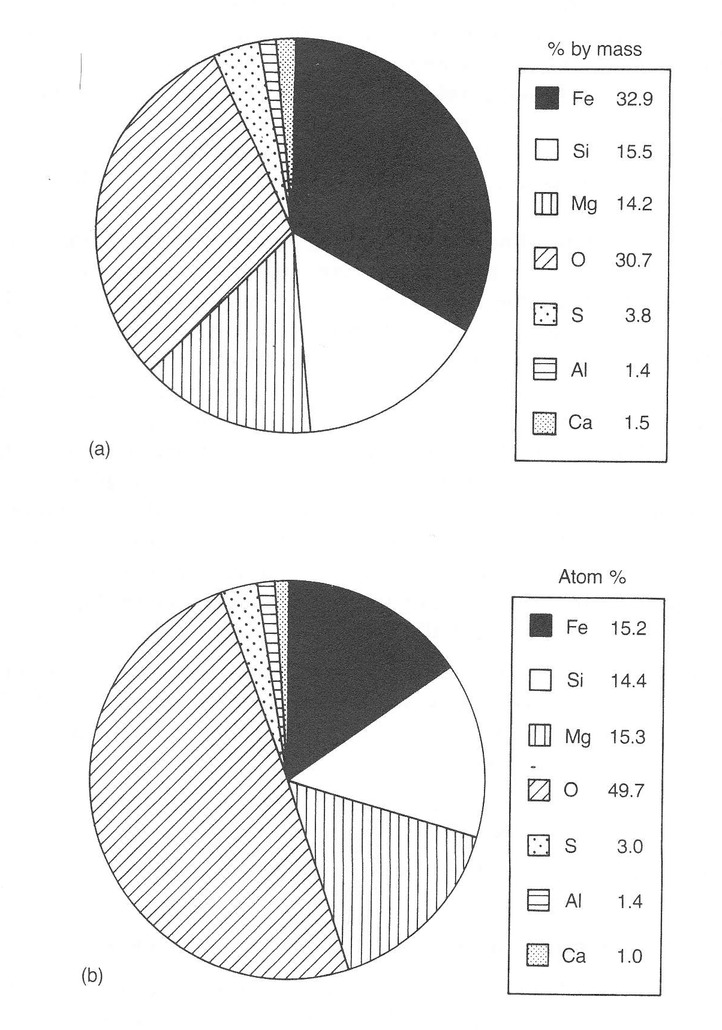
\includegraphics[height=7cm]{images/gravity/brown-musset_fig5-6} \\
{\captionfont
Left:
Element abundance (normalized with $Si=10^6$),
of the solar shallow photosphere compared to
chondritic meteorites (Anders \& Grevesse (1989) \cite{angr89}).
Right:
amounts of Earth's major elements assuming a chondritic
composition (Brown \& Musset (1993) \cite{brmu93}). 
}
\end{center}


The solar-chondritic data in the lefthand frame show that Mg, Fe and Si are 
by far the most abundant (non-volatile) elements.
According to the chondritic Earth hypothesis a similar abundance can be expected
for the bulk-earth.
This is illustrated in the righthand pie diagrams.
Note the large proportion of oxygen, bound in oxides.
In most crust-mantle rocks S is less abundant than Al or Ca.
This is usually explained by assuming that S is relatively volatile and 
also `siderophile', meaning that a significant fraction may have ended up in the
iron-nickle core during an early core-mantle differentiation.

The chondritic meteorites are thought to be representive
of the undifferentiated material condensated from the solar nebula.

Around 1960 a model chemical composition for the bulk of the Earth's
mantle, coined pyrolite,
was introduced by Ringwood (see (Ringwood, 1975) and original references
therein).
This is still used as a reference model.
The pyrolitic composition is associated with the main upper mantle rock type
peridotite that is brought to the Earth's surface in small fragments
included in volcanic rocks (xenoliths) and also in larger,
kilometer sized, fragments in so called peridotite bodies
(Spengler et al., 2006).
The pyrolitic composition of the upper mantle rocks is also strongly
correlated with the composition of chondritic meteorites,
in agreement with the hypothesis of a chondritic origin of the Earth.

Mantle peridotites are found with different degrees of depletion 
(mass fraction lost) by partial melting.
More depleted material is denoted as harzburgite and the relatively 
undepleted peridotite is known as lherzolite.
During progressive partial melting the mineral composition of the residual
rock material, a mineral assemblage consisting of olivine, pyroxene and
garnet, shifts towards the olivine composition.
The olivine enriched harzburgitic residue appears to be the chemical
complement of the basaltic melt product, with respect to the original
lherzolitic mantle source rock.
This depletion relation, between oceanic and continental crust on the one
hand and peridotitic mantle rock on the other,
is reflected in the element abundance of crust and mantle rocks, 
illustrated in the following figure:

\begin{center}
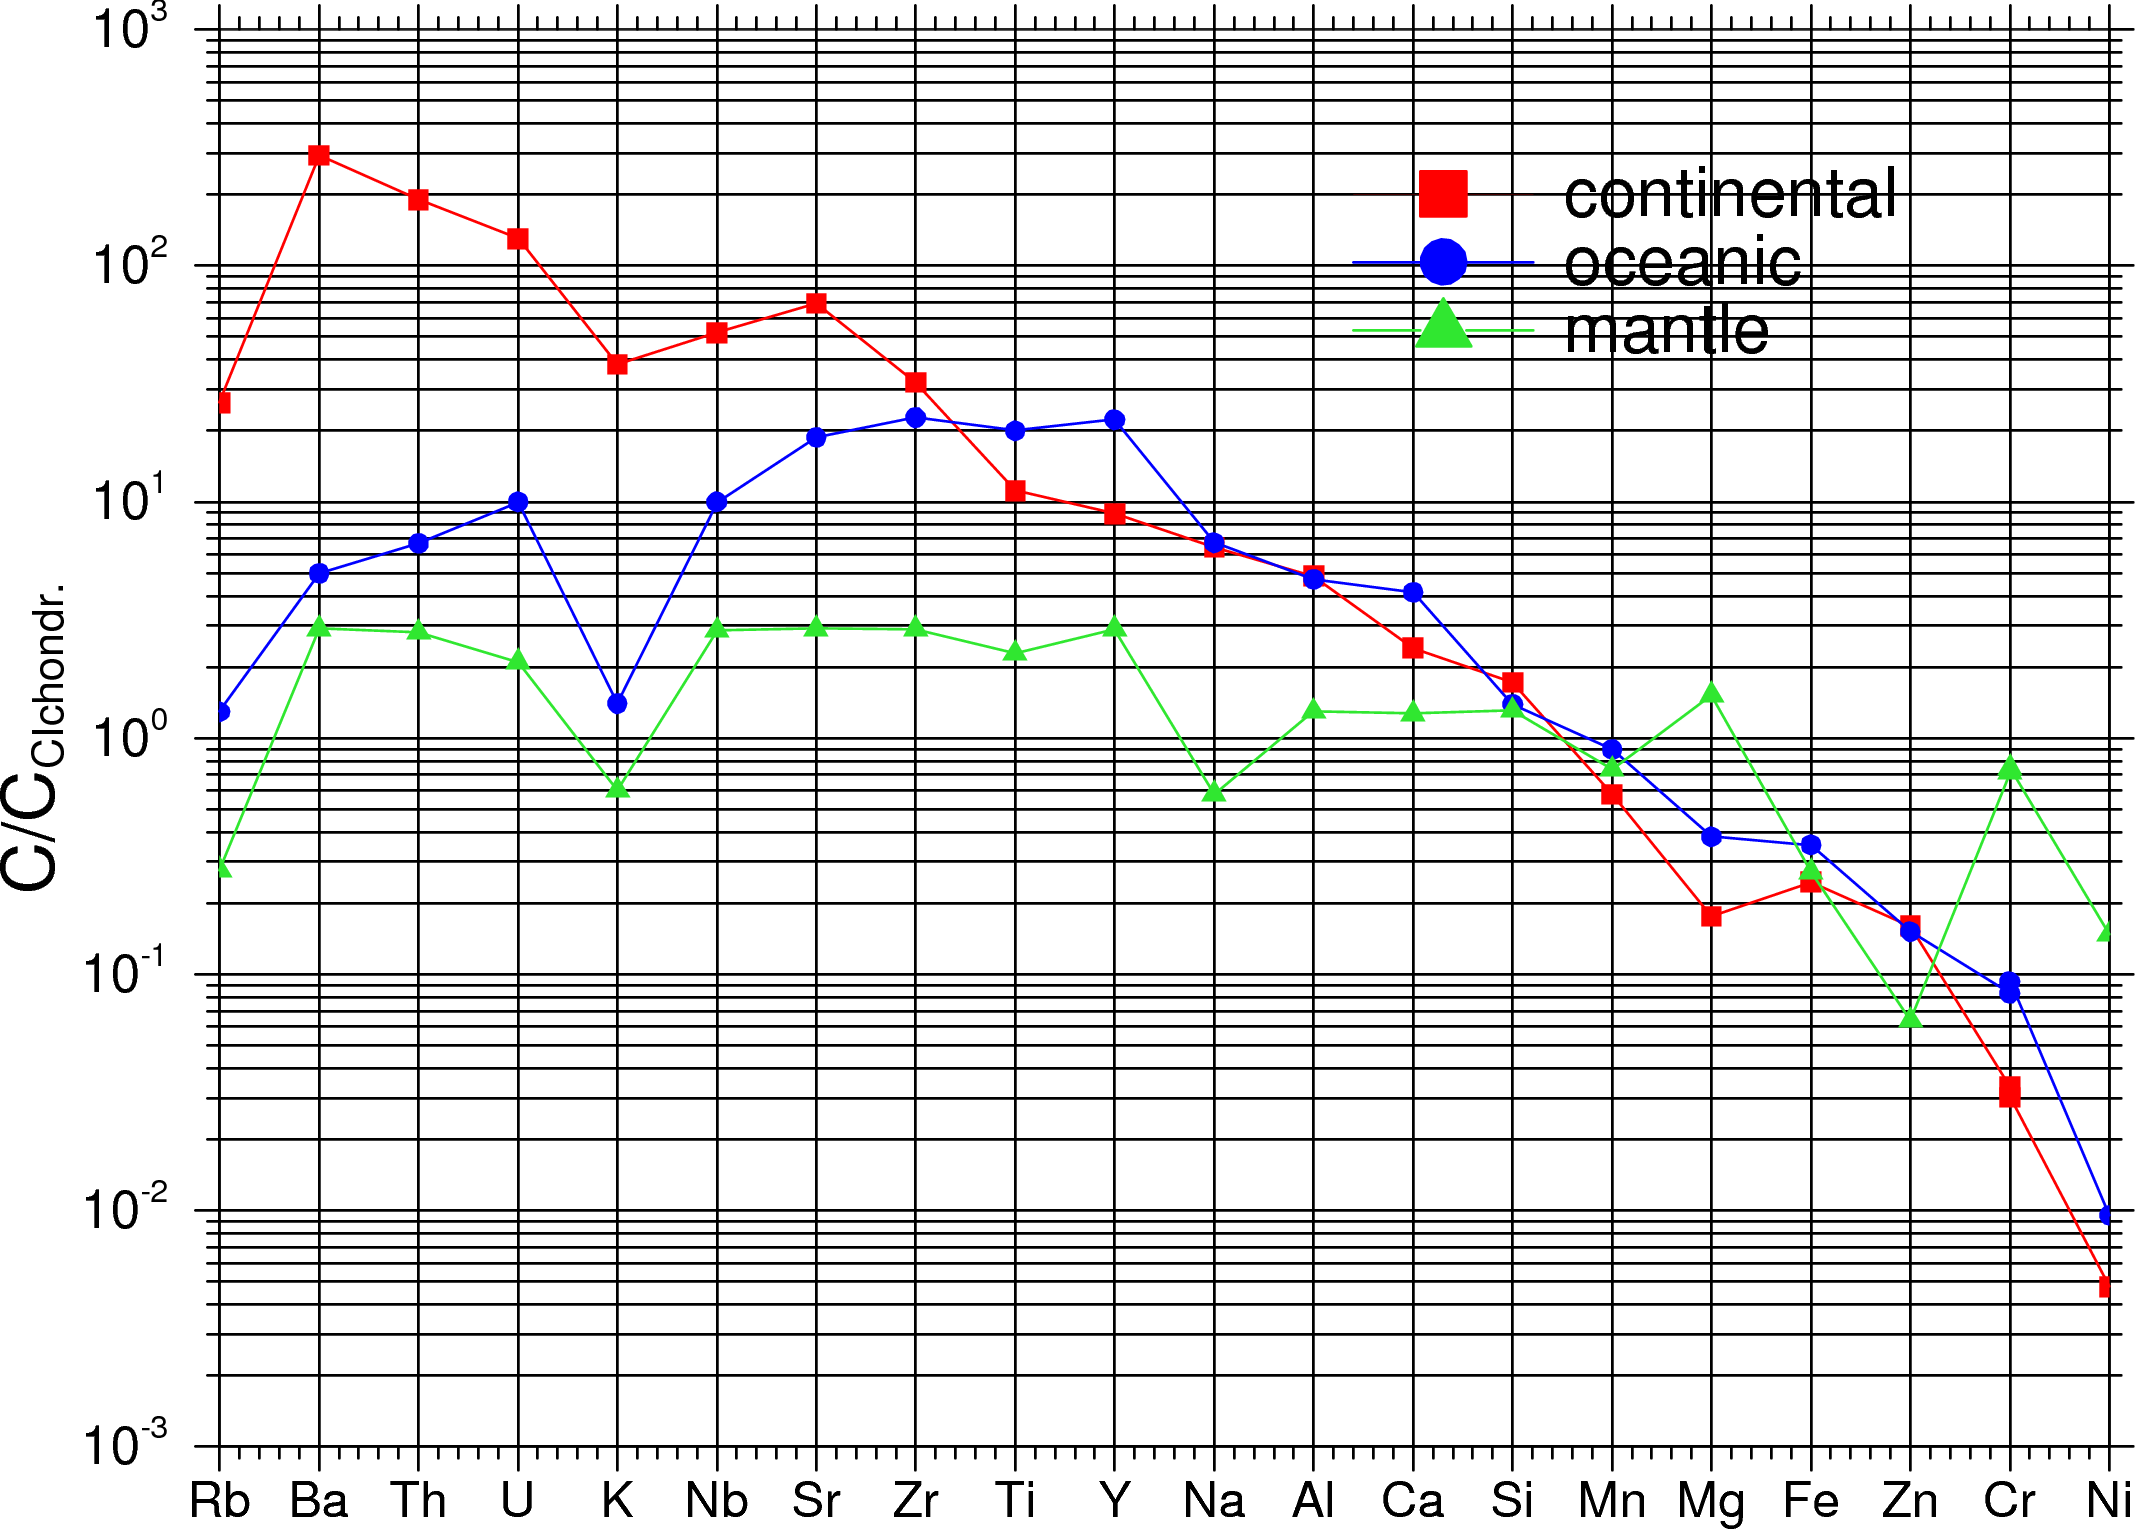
\includegraphics[width=12cm]{images/gravity/abund}\\
{\captionfont 
Chemical abundance of crustal and mantle rocks,
normalized with respect to CI chondritic values.
Data from (McBride and Gilmour, 2003 \cite{mcgi03}).
}
\end{center}

This figure shows abundance ratio's relative to the CI-chondritic composition.
The curve for mantle rock appears to be relatively close to the chondritic composition,
whereas the crustal material is enriched with respect to the mantle in
most elements shown.

A notable exception to this crustal enrichment is found for magnesium which appears
to be enriched in average mantle peridotite.
This is in agreement with the previous observation that 
the olivine/pyroxene content ratio of the residual increases with the
degree of partial melting.
Magnesium content increases with the olivine 
(forsterite $\mathrm{Mg_2SiO_4}$)/pyroxene $\mathrm{MgSiO_3}$ ratio.

An other observation that can be made from the figure above 
is the apparent depletion of the siderophile elements Fe and Ni, both in
crust and mantle material, with respect to the chondritic composition.
This is usually explained by the formation of a liquid Fe, Ni rich metal core
of the Earth during the first few million years of the accretion proces,
in the early solar system.
During this event the molten liquid metal would have differentiated from the 
silicate mantle, leaving the mantle depleted in siderophile (iron loving) elements.

Core formation is also sometimes used as an explanation of the apparent K
(potasium) depletion of both mantle and crust with respect to chondrites.
In this explanation K is disolved in liquid iron in significant quantity
at high pressure and temperature (Rama Murthy et al., 2003).
An alternative explanation for the Earth's K depletion is an escape
of K due to significant volatilization during the planetary accretion proces. 

\fbox{
\begin{minipage}{0.9\textwidth}
\begin{problem}
{\small \it
From Figure \ref{Fig-crust-mantle-data} it can be concluded that the Earth's mantle
and crust lost roughly $2/3$ of its original iron content corresponding to a
chondritic composition.
Verify how this iron-depletion of crust and mantle could be explained by 
differentiation of the Earth's mostly-iron core.
Use the following data in your argument:
a)
The mass fraction of the core $X_c = M_c/M_{\oplus} = 0.315$.
b)
The Fe mass fraction $X_{mFe} \sim 10\%$ of the pyrolitic mantle,
c)
The mass fraction of lighter elements in the core - (S, Si, O)
amounts to about 20\%.
d)
The Fe mass fraction of the bulk Earth $X_{\oplus Fe} ~ \sim 33\%$ 
(Fig. \ref{Fig-photosphere-meteoritic})
}
\end{problem}
\end{minipage}
}
